%%=============================================================================
%% Methodologie
%%=============================================================================

\chapter{\IfLanguageName{dutch}{Methodologie}{Methodology}}%
\label{ch:methodologie}

%% TODO: Hoe ben je te werk gegaan? Verdeel je onderzoek in grote fasen, en
%% licht in elke fase toe welke stappen je gevolgd hebt. Verantwoord waarom je
%% op deze manier te werk gegaan bent. Je moet kunnen aantonen dat je de best
%% mogelijke manier toegepast hebt om een antwoord te vinden op de
%% onderzoeksvraag.

Zoals eerder vermeld zal, dit onderzoek zich focussen op het voorstel dat Bluetooth Low Energy een optimale oplossing is voor asset tracking in de bouwindustrie. Tegenwoordig worden daar vooral andere technologieën voor gebruikt. BLE zit daar reeds tussen, maar in veel mindere mate. In dit gedeelte van de scriptie zal er een requirements-analyse uitgevoerd worden waarin alle functionele en niet-functionele vereisten uitgezocht zullen worden. Vervolgens zal er een long en short list opgesteld worden waarin alle technologieën, die vandaag de dag voornamelijk gebruikt worden, aan bod zullen komen, vergeleken en gefilterd zullen worden op geschiktheid. Hierin zal ook een grondige beschrijving aanwezig zijn van alle voor -en nadelen van BLE. Ook bestaat dit deel uit een toelichting van alle geschikte protocols, software en hardware. Op basis hiervan zal er een experimenteel onderzoek plaatsvinden aan de hand van een zelfontwikkelde Android-applicatie.

\subsection{Requirements-analyse}
Om een correcte vergelijking te maken tussen de meest frequent voorkomende technologieën die gebruikt worden om zaken als machines, voertuigen, werkmateriaal of personeel te traceren op een bouwwerf moet er enkele functionele en niet-functionele vereisten opgelijst worden. Deze zullen de beslissingsfactoren zijn waarom een bepaalde technologie boven een ander wordt verkozen. Aan de hand van deze factoren zal de hierna opgelijste long list geoptimaliseerd worden naar een short list waarin enkel de beste kandidaten nog aanwezig zijn.\\

Voor functionele vereisten gaat er gekeken worden naar zaken die definiëren wat het systeem moet doen om aan de behoeften en verwachtingen van de gebruiker te voldoen. Zaken die hier onder ressorteren zijn bijvoorbeeld het kunnen traceren van een bepaald activum binnen een bepaalde voorafbepaalde radius en een liefst zo klein mogelijke foutmarge hebben tussen de locatie in werkelijkheid en degene aangegeven op de gebruikte software. Dit laatste, ook wel traceernauwkeurigheid genoemd, is een interessant gegeven om te vergelijken aangezien bepaalde technologieën bekend staan om een accuratere plaatsbepaling te hebben dan andere.\\

Voor niet-functionele vereisten gaat er gekeken worden naar zaken die de werking van een systeem kunnen beoordelen, in plaats van specifiek gedrag. Deze eisen staan tegenover de functionele eisen, die hierboven beschreven staan, die specifiek gedrag of functies definiëren. Vereisten die hier ressorteren zijn zaken als initiële en operationele kosten, beveiliging, installatiegemak en het onderhoud van hardware.

\subsection{Long list}
De meest frequent voorkomende technologieën om activa te traceren op een bouwwerf zijn in de literatuurstudie van deze scriptie reeds opgelijst en beschreven geweest. In dit gedeelte van de scriptie zullen deze technologieën met elkaar vergeleken worden aan de hand van functionele en niet-functionele vereisten die in de rubriek hierboven vastgesteld zijn geweest.\\

De zes reeds beschreven technologieën zijn Global Positioning System (GPS), Radio Frequentie Identifier(RFID), Ultra-wideband (UWB), Barcode, QR Codes en Bluetooth Low Energy (BLE). Deze technologieën zullen met elkaar vergeleken worden door middel van volgende functionele en niet-functionele criteria, afgeleid van \textcite{Ahmed2020}:

\begin{itemize}
    \item Werkgebied
    \item Traceernauwkeurigheid
    \item Installatiekosten
    \item Onderhoudskosten
    \item Tag prijs
    \item Functie
\end{itemize}

Uit deze vergelijking zal een kleinere lijst gevormd worden (short list) met de technologieën die het meest potentieel hebben. Deze zullen dan meer in detail bekeken en vergeleken worden welke van de vijf technologieën het meest geschikt is voor de use-case die deze scriptie behandelt namelijk asset tracking op een bouwwerf. Hieruit zal een tijdelijke conclusie opgebouwd worden.\\

\begin{table}
\tiny
\begin{tabularx}{\textwidth} { 
        | >{\raggedright\arraybackslash}X 
        | >{\centering\arraybackslash}X 
        | >{\centering\arraybackslash}X 
        | >{\centering\arraybackslash}X 
        | >{\centering\arraybackslash}X 
        | >{\centering\arraybackslash}X 
        | >{\centering\arraybackslash}X 
        | >{\centering\arraybackslash}X | }
\hline
& GPS & RFID & UWB & Barcode & QR Codes & BLE \\
\hline
Werkgebied & $\infty$ & <100m & <200m & Nvt & Nvt & < 100m\\
Nauwkeurigheid & <10m & <10cm & <30cm & Nvt & Nvt & 2-3m \\
Installatiekosten & Afhankelijk & Duur & Goedkoop & Duur & Goedkoop & Goedkoop \\
Onderhoudskosten & Duur & Goedkoop & Goedkoop & Goedkoop & Goedkoop & Goedkoop  \\
Tag prijs & \euro25 tot \euro50 & 50 cent tot \euro100 & >\euro100 & Afhankelijk & Gratis - afhankelijk & \euro5 tot \euro100 \\
Functie & Identificatie en lokalisatie & Identificatie & Identificatie en lokalisatie & Identificatie & Identificatie & Identificatie en lokalisatie \\
\hline
\end{tabularx}
\caption{Een vergelijking van alle mogelijke asset tracking technologieën volgens bepaalde criteria. De meeste data voor deze tabel werd uit een eerder uitgevoerde studie overgenomen, geschreven door \textcite{Ahmed2020}.}
\label{tab:technologies}
\end{table}

Uit tabel \ref{tab:technologies} kunnen verschillende dingen gelezen en afgeleid worden. Uit deze oppervlakkige verschillen kan al snel een conclusie gemaakt worden welke technologieën meer geschikt zijn dan anderen, hieruit ontstaat dan een specifiekere lijst met kandidaten volgens geschiktheid. \\

\subsubsection{Werkgebied}
Het eerste criterium is werkgebied. Dit toont de afstand waarop een tag bereikt kan worden. Als gekeken wordt naar de verschillende technologieën zijn er meteen zaken die opvallen. Beginnend bij GPS waarbij kan geobserveerd worden dat het werkbereik oneindig is. Dit betekend dat een GPS tag van overal ter wereld bereikt kan worden. Dit is logisch aangezien een GPS tag een simkaart bevat die de positionele en soms ook andere data doorstuurt naar de servers van de gekozen provider over het mobiel netwerk, zoals reeds uitgelegd is geweest. Wat voor dit criteria nog opvalt is dat er bij barcode en QR code 'niet van toepassing' bijstaat. Vanzelfsprekend aangezien barcode en QR code functioneel niet geschikt zijn voor lokalisatie. Barcodes en QR codes kunnen wel van op een afstand gescand worden, maar dit is enkel mogelijk indien er een directe gezichtslijn is met de barcode of QR code. De afstand wordt uiteindelijk bepaald door de resolutie van de barcode of QR code. Als gekeken wordt naar de overige technologieën kan geobserveerd worden dat RFID en BLE gelijk staan en dat UWB het grootste werkgebied heeft. Deze waarden zijn zeker niet vast en kunnen veel afwijken. Dit is data verzameld door \textcite{Roberts2006} en wijkt voor RFID soms honderden meters af van andere data op het internet. Het werkgebied van technologieën als RFID, UWB of BLE hangt dus volledig af van het soort tag. \\

RFID heeft twee soorten tags, namelijk actief en passieve tags. Actieve tags hebben een externe energiebron, meestal een batterij. Dit betekent dat actieve tags van veel verder gelezen kunnen worden. Passieve tags halen hun vermogen uit de transmissie van de lezer via inductieve koppeling \autocite{Roberts2006}. De passieve tags reageren dan op dat signaal. Inductieve koppeling vereist gewoonlijk dat het signaal van redelijk dichtbij verstuurd wordt. Actieve tags langs de andere kant communiceren gewoonlijk via propagatiekoppeling en reageren op de transmissie van de lezer door gebruik te maken van intern vermogen, zoals eerder vermeld.\\

Net zoals bij RFID is het werkgebied van UWB en BLE tags volledig afhankelijk van het soort tag dat gebruikt wordt. In het geval van BLE en UWB wordt het werkbereik bepaald door de combinatie van chipset, antenne en pad verlies. Pad verlies is de maat waarin vermogen van een radiosignaal uitgedrukt wordt dat verloren gaat onderweg van de zender tot de ontvanger \autocite{Tosi2017}. Het wordt gedefinieerd als het verschil tussen het vermogen van de zender en de gevoeligheid van de ontvanger, beiden uitgedrukt in dBm (decibel-milliwatts). Het verband tussen pad verlies en afstand (d) wordt in figuur \ref{fig:range} weergegeven. De vergelijking is wel alleen maar geldig voor een isotrope antenne en houdt geen rekening met eventuele verliezen, reflectie, ruis of obstakels in de omgeving. Het werkgebied kan door deze factoren drastisch variëren. Dit geld natuurlijk voor alle technologieën waar radio frequentie aan te pas komt.\\ 

\begin{figure}
    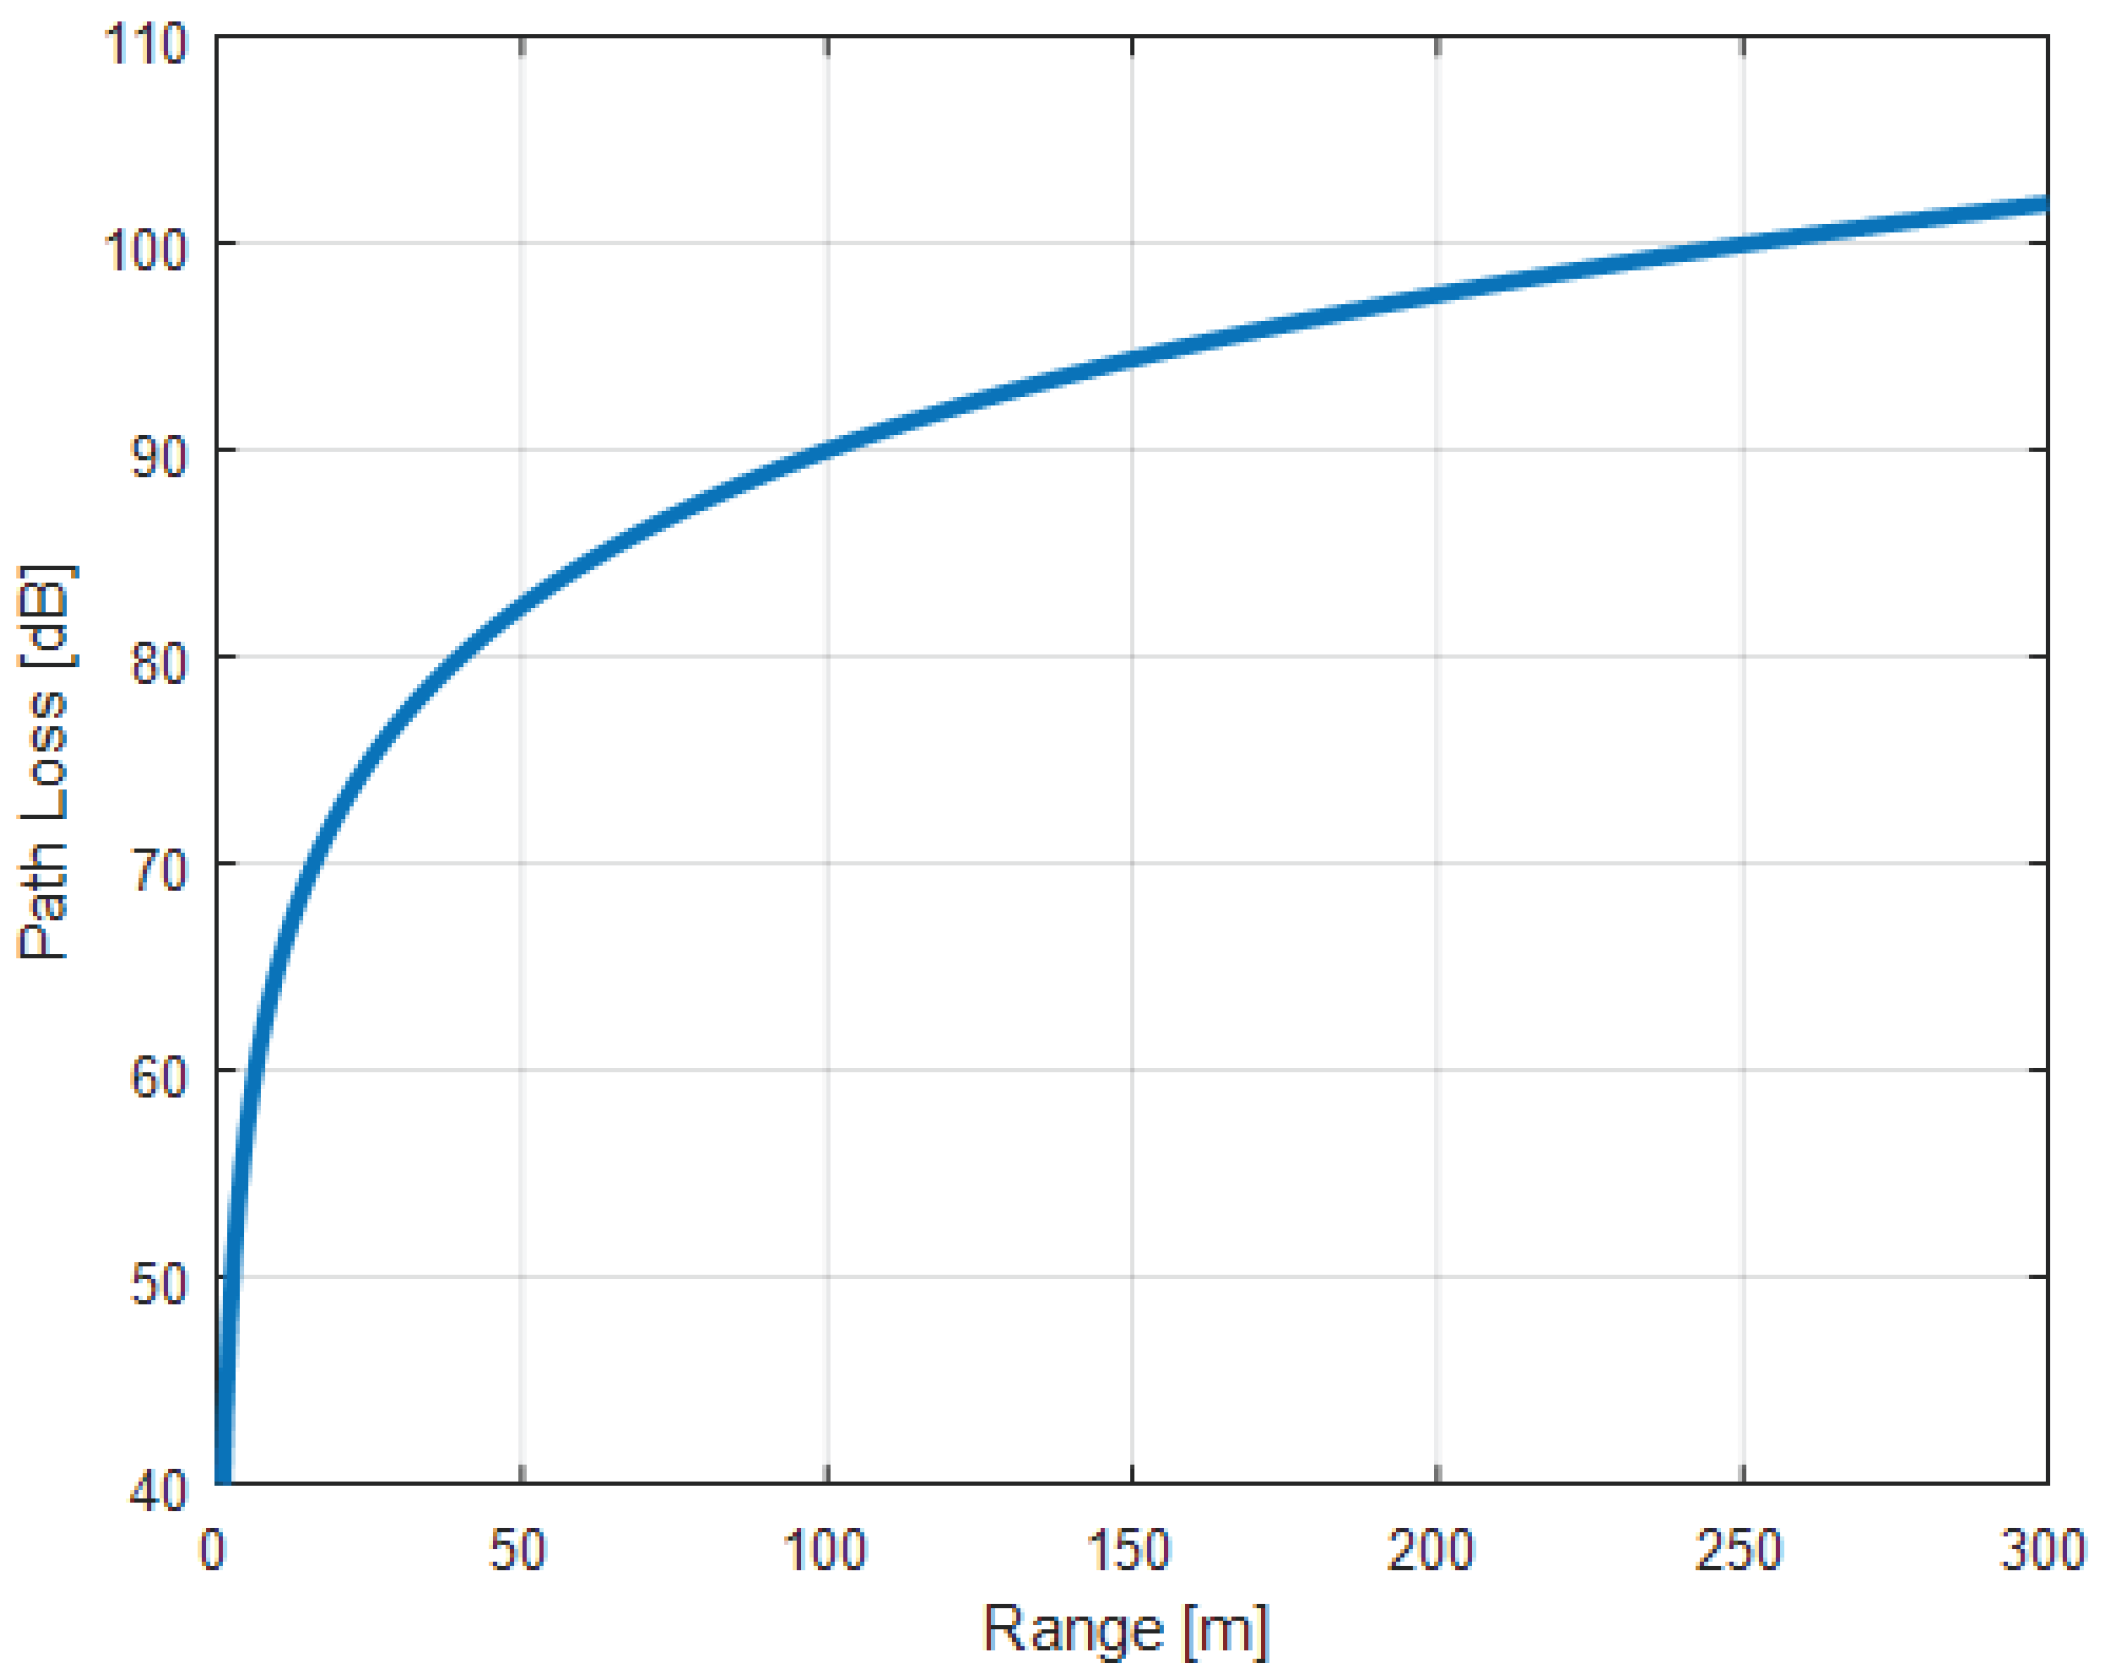
\includegraphics[\textwidth]{range.png}
    \caption[Barcode]{Een grafische representatie van pad verlies, verkregen door vergelijking \ref{pathloss} uit \autocite{Tosi2017}}
    \label{fig:range}
\end{figure}

\begin{equation}
    \label{pathloss}
    pathloss=40+25×log(d)
\end{equation}
\\

\subsubsection{Traceernauwkeurigheid}
Het tweede criterium is traceernauwkeurigheid. Indien een bouwwerf van kleine oppervlakte is of de te traceren activa dicht bij elkaar staan is het van belang dat deze makkelijk gelokaliseerd kan worden en dat deze activa niet met elkaar verwisseld worden door een slechte traceernauwkeurigheid. Aangezien barcode en QR code niet van op afstand traceerbaar zijn zullen deze vanzelfsprekend niet meegerekend worden. De traceernauwkeurigheid bij deze twee technologieën zal altijd 100\% zijn aangezien de activa eerst handmatig gelokaliseerd moet worden voor de code gescand kan worden.\\

De waarden van de andere technologieën zijn vrij verschillend. De technologie die er een beetje uitsteekt is GPS. Dit is geweten dat GPS in het algemeen het minst exact de locatie van iets weergeeft. De afstand kan variëren van een paar meter tot precies. Zo een afwijking kan veroorzaakt worden door verschillende zaken zoals satellietgeometrie, signaal obstructie of atmosferische omstandigheden.\\

Bij de andere technologieën is er nog maar één technologie dat meer dan een meter afwijkt en dit is BLE. Om de afstand te bepalen tussen een zendende (TX) en een ontvangende (RX) node wordt bij BLE Received Signal Strength Indicator (RSSI) gebruikt. Dit is de reden voor de afwijking bij de traceernauwkeurigheid van BLE. Dit is niet de meest accurate manier om de afstand tussen twee nodes te berekenen aangezien dit getal, zoals eerder besproken, door veel zaken beïnvloed kan worden zoals reflectie, ruis of obstakels in de omgeving. RSSI wordt berekend aan de hand van vergelijking \ref{rssi}.

\begin{equation}
    \label{rssi}
    RSSI=−10×N×log(d)+a
\end{equation}\\

Hierin is $N$ een constante die als één wordt aangenomen, $d$ de afstand in meters tussen de twee apparaten en $a$ het vermogen van de TX op één meter afstand.\\

De overige technologieën, RFID en UWB zijn redelijk gelijkend. Beiden hebben maar een mogelijke afwijking van enkele centimeters met RFID als koploper met een mogelijke afwijking onder de tien centimeter.\\

\subsubsection{Installatiekosten}
Installatiekosten zijn de kosten die gemaakt worden bij het installeren van het volledige systeem zoals tags, readers, etc. Bij de zes technologieën zijn er drie die uitspringen, namelijk GPS, RFID en barcode. In het geval van GPS is dit afhankelijk. GPS tags worden aangekocht bij een provider. De tags hangen samen met een uitgebreid systeem dat ervoor zorgt dat de locatie van de tags weergegeven worden op een website of app van de provider. Het is dus afhankelijk van de provider hoeveel installatiekosten zijn voor GPS trackers.\\

In het geval van RFID is het wat anders. RFID tags op zichzelf kunnen zeer goedkoop zijn. De prijs kan van vijftig cent oplopen tot honderd euro. Hier wordt later nog over uitgebreid. Het belangrijkste zijn de zaken als mobiele lezers zoals op figuur \ref{fig:rfidhandheld} of gateways. De prijs van deze zaken kunnen de installatiekosten heel erg doen laten oplopen. Dit is uiteraard vergeleken met de andere technologieën.\\

Barcode is soortgelijk met RFID. Dit is geen technologie waar gewoonweg wat tags voor aangekocht moeten worden en op wat voorwerpen moeten bevestigd worden. De installatiekosten voor barcode wordt stevig omhoog gedreven door de hardware, printer(s) voor barcode labels te printen en de software die nodig is om alles te kunnen traceren. Software wordt hier meegeteld bij de installatiekosten aangezien dit meestal vasthangt aan de hardware.\\

De overige technologieën zijn zeer goedkoop op vlak van installatie. BLE en UWB tags zijn beide plug and play. Dit wil zeggen dat eender wie zulke tags kan aankopen en installeren. Het enigste dat dan nog gedaan moet worden, zijn die tags koppelen aan de software, maar dit staat hier los van aangezien deze technologie gestandaardiseerd is. Indien de assets op een kaart visueel gerepresenteerd moeten worden en gebruik gemaakt wordt van een smartphone zal er waarschijnlijk nog gebruik moeten gemaakt worden van BLE gateways. Aangezien een smartphone de locatie van een BLE tag niet kan afleiden aan de hand van de RSSI waarde zullen er meerdere BLE gateways moeten geïnstalleerd worden die data doorsturen waardoor dit wel mogelijk is. Dit zal de kostprijs ook omhoog drijven indien deze functionaliteit gewest is. \\

In het geval van QR codes is er een verschil tussen de twee soorten QR codes. Zoals eerder besproken is zijn er twee soorten QR code, namelijk statische en dynamische codes. Statische QR codes worden meestal niet gebruikt voor doeleinden als het openen van een link aangezien de URL achter de QR code nooit meer veranderd kan worden. Indien dit wel het geval is, is er geen verschil tussen de twee. Een QR code laten generen is gratis. Dit kan gedaan worden op zeer veel sites online. Hetgeen wat geld kan kosten en bij de installatie, maar ook bij de onderhoudskosten hoort zijn de registratiekosten die vanaf de aankoop maandelijks of jaarlijks betaald moet worden. De prijs hiervan is afhankelijk van het gekozen top-leven domein. \\

\subsubsection{Onderhoudskosten}
Het volgende criterium is onderhoudskosten. Deze term bevat alle kosten die gemaakt worden om het asset tracking systeem werkende te houden. Er is één technologie die hier uitsteekt en dat is GPS. Dit is één van de grootste nadelen van GPS, de onderhoudskosten. Aangezien een asset tracking systeem gebruik makend van GPS zo goed als altijd via een provider gaat, moet deze ook maandelijks betaald worden. Dit kan serieus oplopen in vergelijking met andere technologieën die zo goed als geen onderhoudskosten hebben. \\

Als er gekeken wordt naar technologieën als BLE. De enigste onderhoudskosten die hier zou kunnen voorvallen is de batterij die vervangen zou moeten worden of indien een tag kapot gaat. Dit zijn zaken die niet frequent voorvallen met gevolg dat er voor BLE en UWB, aangezien dat een soortgelijke situatie is, bijna geen onderhoudskosten aan verbonden zijn.\\

In het geval van RFID en barcode zijn de onderhoudskosten net zoals bij BLE en UWB beperkt. Buiten de batterijen van de tags, de tags zelf en de readers in het geval van RFID en de hardware als printers en scanner in het geval van barcode zijn er niet veel onderhoudskosten aan verbonden.\\

In het geval van QR code zijn er zo goed als geen onderhoudskosten aan verbonden buiten als een QR code beschadigd raakt en deze vervangen zou moeten worden.

\subsubsection{Tag prijs}
Tag prijs is vanzelfsprekend de kostprijs van een tag. Dit is een belangrijk gegeven om te vergelijken aangezien dit de onderhoudskosten en initiële kostprijs aanzienlijk kan laten stijgen. De tag is ook meestal de grootste investering bij installeren van een asset tracking systeem. Als gekeken wordt naar de verschillende technologieën is er maar één technologie die er iets of wat uitspringt. Dit is UWB. De enigste technologie waarvan de kostprijs van tags gemiddeld meer dan \euro100 is. Dit prijskaartje is vooral te danken aan de kost van de interne onderdelen van een UWB tag.\\

De mogelijk goedkoopste technologie is RFID. Een passieve RFID tag kan zo goedkoop zijn als tien tot vijftig cent per tag. Indien die tag op metaal moet kunnen werken is dit dan weer duurder. Actieve RFID tags zijn niet goedkoop en kunnen een gemiddelde kostprijs hebben tussen de vijventwintig en honderd euro. Dit komt mede doordat een actieve RFID tag een batterij heeft dat de complexiteit van de tag verhoogt en een groter werkgebied heeft.\\

Bluetooth Low Energy is nog een technologie die bekend staat voor de lage kostprijs van tags. Een BLE tag kan een kostprijs hebben tussen de vijf en honderd euro. De reden zo een drastisch prijsverschil is gelijkaardig als die van RFID tags. Bij een BLE tag draait dit vooral rond het werkgebied of anders gezegd de maximumafstand dat de tag kan bereiken. Dit wordt beïnvloed door de batterij en antenne. De duurdere BLE tags hebben een grotere batterij met een zwaardere antenne die verder signalen kan uitzenden. Hierdoor verhoogt de complexiteit van de tag en drijft dit de kostprijs omhoog.\\

De prijs van barcodes is afhankelijk van de manier waarop de initiële investering gebeurd is. Indien bij de installatie van het barcode systeem printers aangekocht en geïnstalleerd zijn geweest is het printen van een barcode na de initiële aankoop van de hardware zo goed als gratis. Dit is uiteraard exclusief de operating kosten van de printers en de labels waarop de barcodes gedrukt worden. Als deze initiële investering niet gebeurd is geweest zullen alle barcodes bij een extern bedrijf aangekocht moeten worden. \\

In het geval van QR code is de kostprijs voor een code zelf gratis. Zoals eerder vermeld heeft een QR code genereren geen prijskaartje. Dit kan gedaan worden op veel sites online. Wat dus wel eventueel wat geld kan kosten is de prijs van het domein indien de QR code een link opent, maar dit hoort uiteraard niet meer bij de prijs van de QR code zelf. \\

GPS tags kosten gemiddeld tussen de 25 en 50 euro. Vergeleken met de andere technologieën blijkt deze kostprijs zowat in de middenmoot te zitten. De kostprijs van een GPS tracker/tag kan variëren door de gekozen provider en of de tracker/tag extra functionaliteiten heeft zoals de mogelijkheid om extra data door te sturen samen met de locatie.

\subsubsection{Functie}
De laatste criterium is de functie van de technologieën. Aan de hand van dit criterium kan makkelijk bepaald worden wat de mogelijkheden zijn van een bepaalde technologie. Iedere technologie blijkt de mogelijkheid tot identificatie te hebben maar wat voor dit vergelijkend onderzoek belangrijk is, is of de technologie mogelijkheid biedt tot lokalisatie. Als de technologieën overlopen worden springen er meteen twee technologieën uit. Dit zijn barcode en QR code. Bij deze twee is het niet mogelijk om op een of andere manier de locatie van het activa waaraan de code bevestigd is te lokaliseren. Voor de onderzoeksvraag van deze scriptie is het wel van cruciaal belang dat dit mogelijk is en daarom zullen deze twee technologieën achterwegen gelaten worden voor deze vergelijkende studie.\\

\subsection{Short list}
Twee technologieën zijn duidelijk niet geschikt voor asset tracking op een bouwwerf, namelijk barcode en QR code. De reden hiervoor is dat activa waarop een code bevestigd is niet van op afstand gelokaliseerd kan worden. Dit is van cruciaal belang indien men snel activa wil lokaliseren in een complexe en drukke omgeving als een bouwwerf. Indien de overgebleven technologieën nog eens naast elkaar gelegd worden komen we bij tabel \ref{tab:technologies2} uit. Hier zijn er wat extra criteria bijgevoegd aangezien de technologieën op specifiekere vlakken met elkaar verschillen die in de praktijk minstens even belangrijk zouden kunnen zijn om de meest geschikte technologie voor asset tracking op een bouwwerf te kiezen. Dit zijn zaken zoals de levensduur van batterijen, energieverbruik en of de technologie compatibel is met smartphones.

\begin{table}
    \tiny
    \begin{tabularx}{\textwidth} { 
            | >{\raggedright\arraybackslash}X 
            | >{\centering\arraybackslash}X 
            | >{\centering\arraybackslash}X 
            | >{\centering\arraybackslash}X 
            | >{\centering\arraybackslash}X 
            | >{\centering\arraybackslash}X 
            | >{\centering\arraybackslash}X 
            | >{\centering\arraybackslash}X | }
        \hline
        & GPS & RFID & UWB & BLE \\
        \hline
        Functie & Identificatie en lokalisatie & Identificatie & Identificatie en lokalisatie & Identificatie en lokalisatie \\
        Werkgebied & $\infty$ & <100m & <200m & < 100m\\
        Nauwkeurigheid & <10m & <10cm & <30cm & 2-3m \\
        Installatiekosten & Goedkoop & Duur & Goedkoop & Goedkoop \\
        Onderhoudskosten & Duur & Goedkoop & Goedkoop & Goedkoop  \\
        Tag prijs & \euro25 tot \euro50 & 50 cent tot \euro100 & >\euro100 & \euro5 tot \euro100 \\
        \hline
        Batterij & <3 jaar & 3-5 jaar & <2 jaar & 2-5 jaar \\
        Energieverbruik & Laag & Laag/Hoog & Laag & Laagst\\
        Smartphone compatibiliteit & $\bullet$ & & $\bullet$ & $\bullet$ \\
        \hline
    \end{tabularx}
    \caption{Een nauwkeurigere vergelijking van verschillende geschikte asset tracking technologieën volgens bepaalde criteria. De data voor deze tabel werd net zoals bij tabel \ref{tab:technologies} uit een eerder uitgevoerde studie overgenomen, geschreven door \textcite{Ahmed2020}.}
    \label{tab:technologies2}
\end{table}

\subsubsection{Batterij}

De batterij van de technologieën wordt vergeleken met elkaar op basis van hoelang zo een batterij meegaat. De technologie die hier het minst behaalt is UWB. De batterij van de gemiddelde UWB tag gaat minder dat twee jaar mee. Dit is een drastisch verschil indien we dit vergelijken met een technologie als passieve RFID of BLE. Hier kan de levensduur van een batterij wel tot vijf jaar gaan. Dit is meer dan het dubbele van UWB. Als dit voor een langere termijn bekeken wordt kan dit een drastisch verschil in onderhoudskosten geven. \\

GPS blijkt van alle technologieën die vergeleken worden in de middenmoot te zitten met een batterijlevensduur van rond de drie jaar.\\

Uiteraard kunnen deze waarden variëren door verschillende factoren. De belangrijkste factor hierin is hoe groot de batterij is. Het is wel niet altijd zo dat hoe groter de batterij, hoe langer de tag blijft meegaan. Dit kan beïnvloed worden door de zwaarte van de antenne waardoor er meer energie geconsumeerd wordt. Er zijn ook nog externe factoren zoals temperatuur, etc. Batterijen staan bekend om een verminderde levensduur te hebben door lage temperaturen.

\subsubsection{Energieverbruik}

De koploper op het vlak van energieverbruik is Bluetooth Low Energy. Deze specificatie is speciaal ontworpen om een zo laag mogelijk energieverbruik te hebben zonder veel andere functionaliteiten op te geven of limiteren. Dit heeft als gevolg dat BLE een van de beste resultaten behaald op het vlak van batterijlevensduur. Bij de andere technologieën is het enkel RFID dat geen laag energieverbruik heeft. Specifiek zijn dit de actieve RFID tags die een hoog energieverbruik hebben.

\subsubsection{Smartphone compatibiliteit}
Smartphone compatibiliteit is zeer handig voor asset tracking. Dit kan de kosten merkwaardig naar beneden drijven doordat er buiten tags, beacons of gateways geen andere hardware nodig is. Dit is zeker voordelig aangezien iedereen tegenwoordig een smartphone heeft en daarvoor geen extra kosten moeten gerekend worden. Zoals eerder besproken ondersteunen smartphones bijna alle technologieën die hier vergeleken worden. Zoals te zien is op de tabel is de enigste technologie dat niet volledig compatibel is met een smartphone is RFID. Near Field Communication (NFC) is een soort RFID technologie die wel compatibel is met een smartphone. Dit is de technologie die gebruikt wordt voor contactloos betalen. De NFC lezer in een smartphone kan gebruikt worden als RFID lezen voor High Frequentie (HF) RFID tags. De tags die voor asset tracking gebruikt worden zijn Ultra High Frequentie (UHF) RFID tags. Deze tags kunnen niet gelezen worden door de NFC lezer van een smartphone.

\subsection{Conclusie vergelijkende studie}
Uit deze vergelijkende studie kunnen er meteen verschillende zaken geconcludeerd worden. Barcode en QR code zijn geen goede opties voor het gebruik ervan op een bouwwerf. Aangezien de hoofdfunctionaliteit van een asset tracking systeem op een bouwwerf actieve lokaliseren van op een afstand is komen deze twee technologieën hier niet voor in aanmerking.
RFID valt hierdoor ook uit de boot. Het zou mogelijk kunnen om RFID als technologie te gebruiken voor asset tracking op een bouwwerf maar komt toch tekort bij sommige criteria in vergelijking met andere technologieën. Bluetooth Low Energy heeft voor de meeste criteria zeker hoog gescoord samen met UWB en GPS. Hier zal meer afgewogen moeten worden welk criteria belangrijker zijn dan anderen.

\subsection{Voordelen Bluetooth Low Energy}
Na deze vergelijkende studie is er een vrij duidelijk beeld weergegeven wat de voordelen en nadelen van iedere technologie waren in de context van asset tracking op een bouwwerf. Indien Bluetooth Low Energy even geviseerd wordt kunnen we ook deze makkelijk opsommen.\\

Het grootste voordeel van Bluetooth Low Energy is zijn energieverbruik. Zoals reeds besproken is geweest, is de BLE-specificatie hierrond gebouwd. Indien dit vergeleken wordt met technologieën die ook in aanmerking kwamen kan dit een groot verschil betekenen op het vlak van onderhoudskosten aangezien er minder batterijen zullen moeten vervangen worden.\\

Nog een groot voordeel is de kostprijs van tags en andere BLE-gestuurde apparaten. Dit is een zeer belangrijk gegeven aangezien dit de voornaamste kost is bij de installatie van een asset tracking systeem. Prijsverschil op het vlak van tags kan de initiële kostprijs opmerkelijk opdrijven.\\

\subsection{Nadelen Bluetooth Low Energy}
Door een grondige literatuurstudie en een vergelijkende studie zijn er ook wat nadelen naar boven gekomen, vooral in verband met asset tracking en smartphone compatibiliteit.\\

Bluetooth Low Energy is volledig compatibel met zo goed als alle toestellen die in de laatste tien jaar zijn uitgekomen. Het is ondertussen een volgroeide, makkelijk implementeerbare technologie. Maar door de huidige implementatie van Bluetooth Low Energy bij smartphones is het niet mogelijk om te zien vanuit welke richting een signaal komt. Dit wordt niet ondersteund, wat in de toekomst waarschijnlijk wel zo zal zijn. Dit betekend natuurlijk wel een hoop beperkingen indien BLE als asset tracking technologie gebruikt wordt op een bouwwerf. Hier is natuurlijk een workaround voor door gebruik te maken van gateways maar dit is niet even makkelijk implementeerbaar als andere technologieën als UWB of GPS.\\

Nog een nadeel is het werkbereik en de traceernauwkeurigheid. Dit is vergeleken met andere technologieën niet denderend. Het gemiddelde werkgebied van een gemiddelde tag is rond de honderd meter. Dit kan natuurlijk uitgebreid worden naar een paar honderd meter door gebruik te maken van een zwaardere antenne en batterij zoals eerder besproken. Aan de nauwkeurigheid kan weinig gedaan worden. Voor asset tracking op een bouwwerf is dit net niet te veel speling. Hier is er zelfs nog wat ruimte aangezien GPS vaak gebruikt wordt en deze technologie op sommige momenten zelfs 10 meter speling kan hebben.

\subsection{Proof of Concept}
Om te bewijzen dat Bluetooth Low Energy makkelijk integreerbaar is, is er voor dit onderzoek een simpele Android applicatie ontwikkeld. Dit is gedaan door gebruik te maken van het Xamarin.Android framework. Xamarin.Android maakt deel uit van de Xamarin famalie en wordt gebruikt om native Android applicaties te bouwen gebruik makende van C# en Xamarin. De architectuur is hetzelfde als dat van een native Android applicatie met java. Deze technologie is gekozen op vraag van Aucxis aangezien het bedrijf voornamelijk producten ontwikkeld met behulp van .NET.\\

De applicatie is een simpele implementatie van een Bluetooth Low Energy scanner die de RSSI waarden van toestellen in de omgeving kan lezen. Dit is handig aangezien er zo afgeleid kan worden hoe ver deze toestellen van de smartphone verwijderd zijn.\\

Per rij wordt het MAC-adres en RSSI waarde van een toestel in de buurt weergegeven.

\begin{figure}
    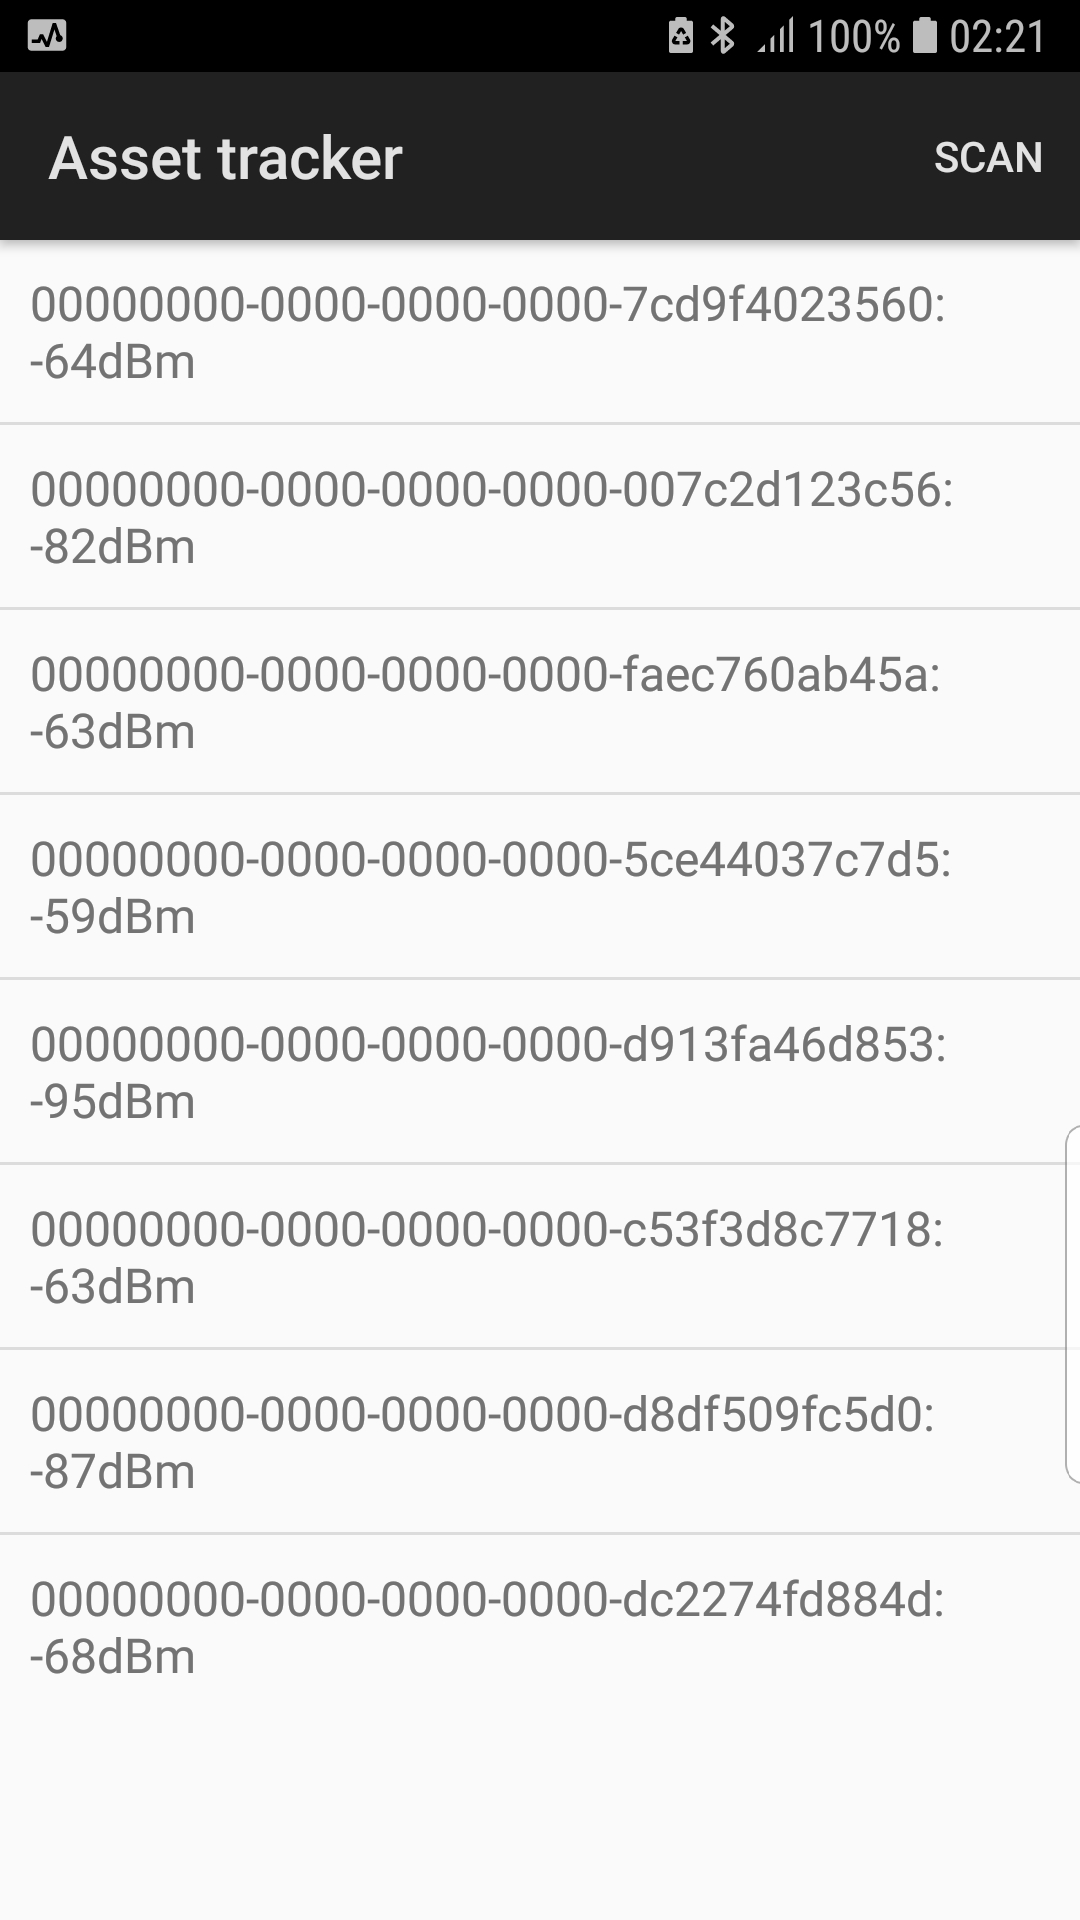
\includegraphics[width=\linewidth]{app.jpg}
    \caption[Asset tracking app]{Screenshot van de zelf ontwikkeld asset tracking app.}
    \label{fig:app}
\end{figure}

\subsubsection{MainActivity}
De app bestaat uit een paar klassen beginnende bij de MainActivity. Dit is wel bekend onder de Android ontwikkelaars. De MainActivity is meestal de activity die het eerst geladen wordt bij het opstarten van de applicatie. In deze applicatie is dit ook de enigste activity.\\

Aangezien de MainAcitivity op de UI-thread draait mag deze niet geblokkeerd worden met scannen naar Bluetooth Low Energy apparaten. Anders zou de hele applicatie blokkeren. We maken in dit geval gebruik van een service. Een bound service om specifiek te zijn. Een bound service is ontworpen zodat een client zoals de MainActivity een client-server interface heeft waarmee zij kunnen interageren. Het scannen naar BLE apparaten gebeurd dus in de service die de MainActivity af en toe eens aanspreekt.\\

De service wordt voornamelijk aangesproken op het moment dat de applicatie opstart en indien een gebruiker om de knop “Scan” drukt.\\

Het aanspreekpunt die door de MainActivity gebruikt wordt om data aan de service te vragen is de BluetoothServiceConnection.

\lstset{%
    language=csharp,  breaklines=true,  numbers=left,
    frame=single, caption={MainActivity.},
    label=code:mainactivity}
\begin{lstlisting}
using Android;
using Android.Content;
using Android.Content.PM;
using Android.Views;

namespace assetdroid
{
    [Activity(Label = "@string/app_name", MainLauncher = true)]
    public class MainActivity : ListActivity
    {
        BluetoothServiceConnection serviceConnection;
        List<string> Devices { get; set; } = new List<string>();
        protected override void OnCreate(Bundle savedInstanceState)
        {
            base.OnCreate(savedInstanceState);
            
            // Set our view from the "main" layout resource
            SetContentView(Resource.Layout.activity_main);
        }
        
        protected override void OnStart()
        {
            base.OnStart();
            if (serviceConnection == null)
            {
                serviceConnection = new BluetoothServiceConnection(this);
            }
            Intent serviceToStart = new Intent(this, typeof(BluetoothService));
            BindService(serviceToStart, serviceConnection, Bind.AutoCreate);
            
            
        }
        
        public override bool OnCreateOptionsMenu(IMenu menu)
        {
            MenuInflater.Inflate(Resource.Menu.top_menus, menu);
            return base.OnCreateOptionsMenu(menu);
        }
        
        public override bool OnOptionsItemSelected(IMenuItem item)
        {
            if (item.TitleFormatted.ToString() == "Scan")
            {
                ScanButtonPressed();
            }
            return base.OnOptionsItemSelected(item);
        }
        
        public async Task UpdateUiForBoundService()
        {
            CheckPermissions();
            var devices = await serviceConnection.Binder.GetBluetoothScanResults();
            
            foreach (var device in devices)
            {
                Devices.Add(device.Id.ToString() + ": " + device.Rssi.ToString() + "dBm");
            }
            
            ListAdapter = new ArrayAdapter<string>(this, Resource.Layout.list_item, Devices);
            
            ListView.TextFilterEnabled = true;
            
            ListView.ItemClick += delegate (object sender, AdapterView.ItemClickEventArgs args)
            {
                Toast.MakeText(Application, ((TextView)args.View).Text, ToastLength.Short).Show();
            };
        }
        
        public void UpdateUiForUnboundService()
        {
            
        }
        
        public async void ScanButtonPressed()
        {
            var devices = await serviceConnection.Binder.GetBluetoothScanResults();
            Devices.Clear();
            foreach (var device in devices)
            {
                Devices.Add(device.Id.ToString() + ": " + device.Rssi.ToString() + "dBm");
            }
            ListAdapter = new ArrayAdapter<string>(this, Resource.Layout.list_item, Devices);
        }
        
        private void CheckPermissions()
        {
            var allowed = CheckSelfPermission(Manifest.Permission.AccessFineLocation);
            if (allowed == Permission.Denied)
            {
                string[] permissions = new string[] { Manifest.Permission.AccessFineLocation };
                RequestPermissions(permissions, 0);
            }
            var again = CheckSelfPermission(Manifest.Permission.AccessFineLocation);
        }
    }
}
\end{lstlisting}
\subsubsection{BluetoothServiceConnection}
De BluetoothServiceConnection verbindt de client met de BluetoothBinder die in de volgende rubiek geïntroduceerd wordt. De BluetoothServiceConnection is ook verantwoordelijk voor de MainActivity op de hoogte te stellen indien de BluetoothService correct geïnstantieerd en/of verbonden is.

\lstset{%
    language=csharp,  breaklines=true,  numbers=left,
    frame=single, caption={BluetoothServiceConnection.},
    label=code:bluetoothserviceconnection}
\begin{lstlisting}
    using Android.Content;
    using Android.OS;
    using Plugin.BLE.Abstractions.Contracts;
    
    namespace assetdroid
    {
        public class BluetoothServiceConnection : Java.Lang.Object, IServiceConnection
        {
            public bool IsConnected { get; set; }
            public BluetoothBinder Binder { get; set; }
            MainActivity mainActivity;
            public BluetoothServiceConnection(MainActivity activity)
            {
                IsConnected = false;
                Binder = null;
                mainActivity = activity;
            }
            
            public void OnServiceConnected(ComponentName name, IBinder service)
            {
                Binder = service as BluetoothBinder;
                IsConnected = Binder != null;
                
                if (IsConnected)
                {
                    mainActivity.UpdateUiForBoundService();
                }
                else
                {
                    mainActivity.UpdateUiForBoundService();
                }
            }
            
            public void OnServiceDisconnected(ComponentName? name)
            {
                IsConnected = false;
                Binder = null;
                mainActivity.UpdateUiForUnboundService();
            }
            
            public async Task<List<IDevice>> GetBluetoothScanResults()
            {
                if (!IsConnected)
                {
                    return null;
                }
                
                return await Binder?.GetBluetoothScanResults();
            }
        }
    }
\end{lstlisting}
\subsubsection{BluetoothBinder}
De BluetoothBinder is een kleine klasse die de BluetoothServiceConnection met de effectieve BluetoothService verbindt. Hier zullen ook de methodes beschreven staan die gebruikt mogen worden door de client aangezien de BluetoothServiceConnection, die in verbinding staat met de Binder, het enige aanspreekpunt is.
\lstset{%
    language=csharp,  breaklines=true,  numbers=left,
    frame=single, caption={BluetoothBinder.},
    label=code:bluetoothbinder}
\begin{lstlisting}
    using Android.OS;
    using Plugin.BLE.Abstractions.Contracts;
    
    namespace assetdroid
    {
        public class BluetoothBinder : Binder
        {
            public BluetoothService Service { get; set; }
            public BluetoothBinder(BluetoothService service)
            {
                Service = service;
            }
            
            public async Task<List<IDevice>> GetBluetoothScanResults()
            {
                return await Service?.GetBluetoothScanResults();
            }
        }
    }
\end{lstlisting}
\subsubsection{BluetoothService}
De BluetoothService is de effectieve service die gaat scannen naar Bluetooth Low Energy apparaten. Deze service draait op de achtergrond en werk asynchroon. Voor het scannen naar BLE apparaten is gebruik gemaakt van een bibliotheek genaamd \href{https://github.com/dotnet-bluetooth-le/dotnet-bluetooth-le}{Plugin.BLE}. Dit is een Bluetooth Low Energy bibliotheek specifiek voor Xamarin en MAUI.  
\lstset{%
    language=csharp,  breaklines=true,  numbers=left,
    frame=single, caption={BluetoothService.},
    label=code:bluetoothservice}
\begin{lstlisting}
using Android.Content;
using Android.OS;
using Plugin.BLE;
using Plugin.BLE.Abstractions.Contracts;
using Plugin.BLE.Android;
using IAdapter = Plugin.BLE.Abstractions.Contracts.IAdapter;

namespace assetdroid
{
    [Service(Name = "com.stefboerjan.BluetoothService")]
    public class BluetoothService : Android.App.Service
    {
        private IBluetoothLE ble;
        private IAdapter adapter;
        private List<IDevice> Devices { get; set; }
        public IBinder Binder { get; private set; }
        
        public override async void OnCreate()
        {
            base.OnCreate();
            ble = CrossBluetoothLE.Current;
            adapter = CrossBluetoothLE.Current.Adapter;
            adapter.ScanTimeout = 2000;
            Devices = new List<IDevice>();
            adapter.DeviceDiscovered += (s, a) => Devices.Add(a.Device);
        }
        
        public override IBinder? OnBind(Intent? intent)
        {
            Binder = new BluetoothBinder(this);
            return Binder;
        }
        
        public override bool OnUnbind(Intent? intent)
        {
            return base.OnUnbind(intent);
        }
        
        public override void OnDestroy()
        {
            ble = null;
            adapter = null;
            Devices = null;
            Binder = null;
            base.OnDestroy();
        }
        
        public async Task<List<IDevice>> GetBluetoothScanResults()
        {
            try
            {
                var state = ble.State;
                Devices.Clear();
                await adapter.StartScanningForDevicesAsync();
                return Devices;
            }
            catch (Exception ex)
            {
                return null;
            }
        }
    }
}
\end{lstlisting}